
\documentclass[en,11pt]{aghdpl}

\usepackage[english]{babel}
\usepackage[utf8]{inputenc}

% dodatkowe pakiety
\usepackage{enumerate}
\usepackage{listings}
\usepackage{framed}
\usepackage{amsmath}
\usepackage{amsfonts}
\usepackage{mathtools}
\usepackage{algorithm}
\usepackage[noend]{algpseudocode}
\lstloadlanguages{TeX}

\lstset{
  literate={ą}{{\k{a}}}1
           {ć}{{\'c}}1
           {ę}{{\k{e}}}1
           {ó}{{\'o}}1
           {ń}{{\'n}}1
           {ł}{{\l{}}}1
           {ś}{{\'s}}1
           {ź}{{\'z}}1
           {ż}{{\.z}}1
           {Ą}{{\k{A}}}1
           {Ć}{{\'C}}1
           {Ę}{{\k{E}}}1
           {Ó}{{\'O}}1
           {Ń}{{\'N}}1
           {Ł}{{\L{}}}1
           {Ś}{{\'S}}1
           {Ź}{{\'Z}}1
           {Ż}{{\.Z}}1
}

%---------------------------------------------------------------------------

\author{Piotr Szmigielski}
\shortauthor{P. Szmigielski}

\titlePL{Implementacja algorytmów dla systemów Monroe i Chamberlina-Couranta z nieliniową funkcją satysfakcji}
\titleEN{Implementation of algorithms for Monroe and Chamberlin-Courant systems under nonlinear satisfaction function}

\shorttitlePL{Implementacja algorytmów dla systemów Monroe i Chamberlina-Couranta z nieliniową funkcją satysfakcji}
\shorttitleEN{Implementation of algorithms for Monroe and Chamberlin-Courant systems under nonlinear satisfaction function}

\thesistype{Master of Science Thesis}

\supervisor{Piotr Faliszewski, PhD}

\degreeprogramme{Computer Science}

\date{2015}

\department{Department of Computer Science}

\faculty{Faculty of Computer Science, Electronics and Telecommunications}


\setlength{\cftsecnumwidth}{10mm}

%---------------------------------------------------------------------------

\usepackage{array}
\newcolumntype{C}[1]{>{\centering\arraybackslash\hspace{0pt}}m{#1}}

\begin{document}

\setcounter{secnumdepth}{3}
\setcounter{tocdepth}{3}
\let\cleardoublepage\clearpage
\def\bibname{References}
\def\listtablename{List of Tables}
\def\tablename{Table}

\newcommand{\abs}[1]{\lvert#1\rvert}
\newcommand{\norm}[1]{\lVert#1\rVert}

\titlepages

\tableofcontents

\chapter{Introduction}
\label{cha:introduction}

We study the effectiveness of algorithms for approximate winner determination under the Monroe and Chamberlin-Courant multiwinner voting rules using nonlinear satisfaction function. Both of the rules aim to select a group of candidates that best represent the voters. Having good voting rules and algorithms for them is important, as multiwinner elections are used both in human societies (e.g. parliament elections) and software systems (e.g. recommendation systems). Rules studied in this paper are particularly interesting because they have both desired features of multiwinner rules: they provide accountability (there is connection between the elected candidates and the voters, so each voter has a representative assigned to her and each candidate knows who she represents) and proportional representation of the voters’ views.

We assume that candidates participate in the election with multiple winners (a commitee with multiple members is selected) and they are elected by voters, each of whom ranks all the candidates (each voter provides a linear order over the set of candidates expressing their preferences). For each voter the Monroe and Chamberlin-Courant rules assign a single candidate as their representative (with some constraints, which are detailed in the further part of the thesis).

The candidates are selected and assigned to the voters optimally, either by maximizing the total satisfaction of all voters, or by minimizing the total dissatisfaction of all voters.
The total satisfaction is calculated as a sum of individual satisfactions of the voters. We assume that there is a  satisfaction function that measures how well a voter is represented by the candidate. The function is the same for each voter. It is a decreasing function, so a voter is more satisfied if the candidate assigned to her is ranked higher. The dissatisfaction is calculated in the similar way, except that the function is an increasing one. In this paper I study cases in which the satisfaction function is a nonlinear one.

The main drawback of the aforementioned rules is that election winner determination is NP-hard under each of them \cite{2} which makes them hard to use in practice, as it would force the use of algorithms that don’t provide an optimal result for every data set. Therefore, using these systems for real-life elections may rise some difficulties. However, they can be used for the recommendation systems conveniently, as a good but not optimal recommendation is still useful. Skowron et al. \cite{1} provided approximation algorithms for both the rules that return near-optimal results for various test cases (including real-life data and synthetic data), but for linear satisfaction function only.

In this paper we focus on providing several algorithms for the Monroe and Chamberlin-Courant rules using nonlinear satisfaction function and evaluating them empirically against various data sets. For smaller data, results can be easily assessed by comparing them to the optimal result (calculated with the brute-force algorithm). For bigger data, the upper bound of the optimal result must be used for comparison. We implement and evaluate various heuristic algorithms, as well as the existing approximation algorithms for the linear satisfaction function, but applying them to the nonlinear cases.


% \chapter{Motivation and Goals}
\label{cha:motivation}

Monroe and Chamberlin-Courant systems may be potentially very useful, because they are one of the few multiwinner election systems that provide both accountability of candidates to the voters (each voter has one particular representative in the elected commitee) and proportional results. Most of the currently used voting rules lack at least one of these properties. For example, D'Hondt method used to elect members of Polish lower house of parliament lacks accountability (voters are accountable to political parties rather than specific parliament members), while single-member constituency plurality system used for United Kingdom parliament elections lacks proportionality.

As finding optimal solution for both of the aforementioned systems is NP-hard \cite{2}, there is a need to provide good algorithms which can compute result which is suboptimal but still as close to optimal as possible. Using such result in real-life elections (e.g. for parliament) is disputable. However, for some software applications, e.g. recommendation systems, it can be used seamlessly.

Skowron et. al \cite{1} have already provided approximation algorithms for these systems, but only under linear satisfaction function. In this thesis we focus on providing algorithms for non-linear satisfaction functions, as they can better reflect real preferences of the voters.
\chapter{Rozdział do testów}

Brak sensownej zawartości ;)



\chapter{State of the Art}
\label{cha:stateArt}
\chapter{Implemented Algorithms}
\label{cha:implementedAlgorithms}

In this chapter we present implemented algorithms for the utilitarian versions of Monroe and Chamberlin-Courant multiwinner voting rules in the satisfaction-based framework.
\\

\noindent
\textbf{Proposition 1 (Implicit in the paper of Betzler et al. \cite{3}).} Let $\alpha$ be a normal DPSF, $N$ be a set of agents, $A$ be a set of alternatives, $V$ be a preference profile of $N$ over $A$, and $S$ a $K$-element subset of $A$ (where $K$ divides $\norm{N}$). Then there is a polynomial-time-algorithm that computes a (possibly partial) optimal K-assignment $\Phi^{S}_{\alpha}$ (Monroe K-assignment $\Phi^{S}_{\alpha}$) of the agents to the alternatives from $S$.
\\

\section{Algorithm A}

Algorithm A was first presented by Skowron et al. \cite{1} and tries to solve $\alpha$-Monroe-SatWinner. It builds a solution iteratively (greedily). In each step we pick some not-yet-assigned alternative $a_{i}$ and assign it to those $\frac{N}{K}$ agents that are not assigned to any other alternative yet and whose satisfaction of being matched with $a_{i}$ is maximal (criterion for picking an alternative in each step is a sum of satisfaction of agents selected this way). This algorithm runs in polynomial time \cite{1}. Pseudocode is presented in Algorithm 1.

\begin{algorithm}
\caption{Algorithm A}\label{euclid}
\begin{algorithmic}[1]
	\Procedure{ComputeMonroeSatWinner}{}
		\State $\Phi \gets$ a map defining a partial assignment, iteratively built by the algorithm
		\State $\Phi^{\leftarrow} \gets$ the set of agents for which the assignment is already defined
		\State $\Phi^{\rightarrow} \gets$ the set of alternatives already used in the assignment
		\If {$K \leq 2$}
			\State compute the optimal solution using an algorithm of Betzler et al. \cite{1} and return
		\EndIf
		\State $\Phi$ = $\{\}$
		\For{$i \gets 1$ to $K$}
			\State $score \gets \{\}$
			\State $bests \gets \{\}$
			\ForAll{$a_{i} \in A \setminus \Phi^{\rightarrow}$}
				\State $agents \gets$ sort $N \setminus \Phi^{\leftarrow}$ so that if agent $j$ preceeds agent $j'$ then $pos_{j}(a_{i}) \leq pos_{j'}(a_{i})$
				\State $bests[a_{i}] \gets$ choose first $\frac{N}{K}$ elements from $agents$
				\State $score[a_{i}] \gets \sum_{j \in bests[a_{i}]}(m - pos_{j}(a_{i}))$
			\EndFor
			\State $a_{best} \gets argmax_{a \in A \setminus \Phi^{\rightarrow}} score[a]$
			\ForAll{$j \in bests[a_{best}]$}
				\State $\Phi[j] \gets a_{best}$
			\EndFor
		\EndFor
	\EndProcedure
\end{algorithmic}
\end{algorithm}

\section{Algorithm B}

Algorithm B is an extension to Algorithm A and was presented in the same paper. The idea is to run Algorithm A first and then optimally reassign the alternatives to the voters (using Proposition 1). It should noticeably improve the results of the algorithm and it still runs in polynomial time.

\section{Algorithm C}

Algorithm C is a further extension to Algorithm B, also presented by Skowron et al. \cite{1}. While Algorithm B only keeps one partial assignment function $\Phi$ that is extended in each step until it becomes a full assignment, Algorithm C stores a list of $d$ functions ($d$ is provided as an algorithm parameter). At each step, for each alternative $a$ with no agent assigned and for each $\Phi$ of the $d$ functions stored, we compute an extension to $\Phi$ that assigns $\frac{N}{K}$ agents (that are not assigned to any other alternative yet) to $a$ (the same way as in Algorithm A). For the next step, $d$ functions that give the highest satisfaction are kept. If we take $d = 1$, we obtain Algorithm B. Pseudocode is presented in Algorithm 3.
\\

Unlike previous algorithms, Algorithm C can be used for both Monroe and Chamberlin-Courant rules. To adapt it to the Chamberlin-Courant rule, we have to replace the contents of the first for all loop with the appropriate code, presented in Algorithm 2.

\begin{algorithm}
\caption{Algorithm C - CC for all code replacement}\label{euclid}
\begin{algorithmic}[1]
	\ForAll{$a_{i} \in A \setminus \Phi^{\rightarrow}$}
		\State $\Phi' \gets \Phi$
		\ForAll{$j \in N$}
			\If{agent $j$ prefers $a_{i}$ to $\Phi'(j)$}
				\State $\Phi'(j) \gets a_{i}$
			\EndIf
		\EndFor
		\State $newPar.push(\Phi')$
	\EndFor
\end{algorithmic}
\end{algorithm}

\begin{algorithm}
\caption{Algorithm C}\label{euclid}
\begin{algorithmic}[1]
	\Procedure{ComputeMonroeSatWinner}{}
		\State $\Phi \gets$ a map defining a partial assignment, iteratively built by the algorithm
		\State $\Phi^{\leftarrow} \gets$ the set of agents for which the assignment is already defined
		\State $\Phi^{\rightarrow} \gets$ the set of alternatives already used in the assignment
		\State $Par \gets$ a list of partial representation functions
		\State $Par = []$
		\State $Par.push(/{/})$
		\For{$i \gets 1$ to $K$}
			\State $newPar = []$
			\For{$\Phi \in Par$}
				\State $bests \gets \{\}$
				\ForAll{$a_{i} \in A \setminus \Phi^{\rightarrow}$}
					\State $agents \gets$ sort $N \setminus \Phi^{\leftarrow}$ (agent $j$ preceeds agent $j'$ implies that $pos_{j}(a_{i}) \leq pos_{j'}(a_{i})$
					\State $bests[a_{i}] \gets$ choose first $\frac{N}{K}$ elements of $agents$
					\State $\Phi' \gets \Phi$
					\ForAll{$j \in bests[a_{i}]$}
						\State $\Phi'[j] \gets a_{i}$
					\EndFor
					\State $newPar.push(\Phi')$
				\EndFor
			\EndFor
			\State sort $newPar$ according to descending order of the total satisfaction of the assigned agents
			\State $Par \gets$ choose first $d$ elements of $newPar$
		\EndFor
		\For{$\Phi \in Par$}
			\State $\Phi \gets$ compute the optimal representative function using an algorithm of Betzler et al. \cite{3} for the set of winners $\Phi^{\rightarrow}$
		\EndFor
		\State \Return the best representative function from $Par$
	\EndProcedure
\end{algorithmic}
\end{algorithm}

\section{Algorithm R}

As shown by Skowron et al. \cite{1}, algorithms A, B and C achieve very high approximations ratios under linear satisfaction function for the cases where $K$ is small relative to $m$. For the other cases, we can use a sampling-based randomized algorithm (called Algorithm R). We expect that under nonlinear satisfaction function algorithms should behave similarly in relation to each other as under a linear one.
\\

Algorithm R randomly picks $K$ alternatives and then, using Proposition 1, assigns them to agents optimally. As such an algorithm may be simply unlucky and pick alternatives that are ranked low, random assignment should be computed a given number of times (which is provided as a parameter), so there is a greater probability to attain a high quality solution. If $K$ is comparable to $m$ then it is likely that generated results would include a solution that is at least close to optimal. Algorithm can naturally be used for both Monroe and Chamberlin-Courant systems.

\section{Algorithm AR}

Algorithm family A-C and algorithm R are naturally suitable for different cases. Therefore, Skowron et al. \cite{1} proposed to combine algorithms A and R into Algorithm AR. They also showed that under linear satisfaction function, Algorithm AR can achieve approximation ratio of $0.715 - \epsilon$ with probability $\lambda$. Both $\epsilon$ and $\lambda$ are provided as algorithm parameters. Naturally, for different satisfaction functions approximation ratio may vary, but we decided to test the algorithm in an unchanged version for comparison. Pseudocode is presented in Algorithm 4.

\begin{algorithm}
\caption{Algorithm AR}\label{euclid}
\begin{algorithmic}[1]
	\Procedure{ComputeMonroeSatWinner}{}
		\State $H_{j}$ is the $j$'th $harmonic number$ $H_{j} = \sum_{i=1}^{j}(\frac{1}{i})$
		\State $\lambda \gets$ probability of achieving the approximation ratio $0.715 - \epsilon$ under linear satisfaction function
		\If{$\frac{H_{K}}{K} \geq \frac{e}{2}$}
			\State compute the optimal solution using an algorithm of Betzler et al. \cite{3} and return
		\EndIf
		\If{$m \leq 1 + \frac{2}{e}$}
			\State compute the optimal solution using a simple brute force algorithm and return
		\EndIf
		\State $\Phi_{1} \gets$ solution computed by Algorithm A
		\State $\Phi_{2} \gets$ solution computed by Algorithm R (sampled $\log (1 - \lambda) \cdot \frac{2 + e}{e}$ times)
		\State \Return the better assignment among $\Phi_{1}$ and $\Phi_{2}$
	\EndProcedure
\end{algorithmic}
\end{algorithm}

\section{Algorithm GM}

Algorithm GM (greedy marginal improvement) is an algorithm that was introduced by Lu and Boutilier \cite{4} for the Chamberlin-Courant rule only. However, it was later generalized by Skowron et al. \cite{1}, so it can be applied to the Monroe rule as well. In the Monroe case, it can be considered as the Algorithm B improvement.
\\

We start with an empty set $S$. In each iteration of the algorithm we select an alternative $a$ that is not assigned to agents yet, and that maximizes the satisfaction value $l_{sum}^{\alpha}(\Phi^{S \cup \{a\}}_{\alpha})$. Iterations are executed until a complete committee is selected, so $K$ iterations are required. For Monroe case, computing $\Phi^{S}_{\alpha}$ is slow (it is achieved by using min-cost/max-flow algorithm \cite{3}), which makes the algorithm execute for a relatively long time. Pseudocode is presented in Algorithm 5.
\\

Algorithm GM is an $1-\frac{1}{e}$-approximation algorithm for any normal IPSF \cite{1,5}.

\begin{algorithm}
\caption{Algorithm GM}\label{euclid}
\begin{algorithmic}[1]
	\Procedure{ComputeSatWinner}{}
		\State $\Phi^{S}_{\alpha}$ - the partial assignment that assigns a single alternative to at most $\frac{n}{K}$ agents, that assigns to the agents only the alternatives from $S$, and that maximizes the utilitarian satisfaction $l^{\alpha}_{sum}(\Phi^{S}_{\alpha})$
		\State $S \gets \emptyset$
		\For{$i \gets 1$ to $K$}
			\State $a \gets argmax_{a \in A \setminus S} l^{\alpha}_{sum} (\Phi^{S \cup \{\alpha\}}_{\alpha})$
			\State $S \gets S \cup \{a\}$
		\EndFor
		\State \Return $\Phi^{S}_{\alpha}$
	\EndProcedure
\end{algorithmic}
\end{algorithm}

\section{Algorithm P}

Algorithm P can only be applied to Chamberlin-Courant problem. It was first introduced by Skowron et al. \cite{1}. In the beginning, it computes $x$ (a non-negative integer). Next, it computes an assignment that should maximize the number of agents that have an alternative from the first $x$ spots in their preferences assigned to them. This process is executed greedily. Afterwards, if there are still agents with no alternative assigned, the best alternative is picked from the ones already selected for at least one other agent.
\\

$w(x)$ used in the algorithm is a Lambert's W-function, defined to be the solution of the equation $x = w(x)e^{w(x)}$. Algorithm runs in polynomial time. Pseudocode of Algorithm P is presented in Algorithm 6.

\begin{algorithm}
\caption{Algorithm P}\label{euclid}
\begin{algorithmic}[1]
	\Procedure{ComputeCCSatWinner}{}
		\State $\Phi \gets$ a map defining a partial assignment, iteratively built by the algorithm
		\State $\Phi^{\leftarrow} \gets$ the set of agents for which the assignment is already defined
		\State $\Phi^{\rightarrow} \gets$ the set of alternatives already used in the assignment
		\State $num\_pos_{x}(a) \gets \norm{\left\{ i \in [n] \setminus \Phi^{\leftarrow} : pos_{i}(a) \leq x \right\}}$ - the number of not-yet assigned agents that rank alternative $a$ in one of their first $x$ positions
		\State $w(\cdot)$ - Lambert's W-function
		\State $\Phi = \{\}$
		\State $x = \left\lceil \frac{mw(K)}{K} \right\rceil$
		\For{$i \gets 1$ to K}
			\State $a_{i} \gets argmax_{a \in A \setminus \Phi^{\rightarrow}} num\_pos_{x}(a)$
			\ForAll{$j \in [n] \setminus \Phi^{\leftarrow}$}
				\If{$pos_{j}(a_{i}) < x$}
					\State $\Phi[j] \gets a_{i}$
				\EndIf
			\EndFor
		\EndFor
		\ForAll{$j \in A \setminus \Phi^{\leftarrow}$}
			\State $a \gets$ such alternative from $\Phi^{\rightarrow}$ that $\forall_{a' \in \Phi^{\rightarrow}} pos_{j}(a) \leq pos_{j}(a')$
			\State $\Phi[j] \gets a$
		\EndFor
		\State \Return $\Phi$
	\EndProcedure
\end{algorithmic}
\end{algorithm}

\section{Genetic Algorithm}

The idea of our algorithm is loosely based on metaheuristic genetic algorithms, such as the firefly algorithm \cite{6}.
\\

Our Genetic Algorithm starts with an initial set of creatures (each of them presenting a possible solution under Chamberlin-Courant rule) which are later mutated and crossed over with each other. The best creatures (ones with the highest total satisfaction) are preferred for further mutation and crossover in order to better investigate the neighbourhood of local maxima, but on the other hand algorithm also produces new creatures by crossing over random existing ones to better explore entire solution space, not limiting to local extrema.
\\

In each iteration of the algorithm creatures are evaluated (satisfaction is computed). Best creature in terms of total satisfaction is compared with currently best found creature and takes its place if it is better. Half of the evaluated creatures (the best ones) are chosen for further propagation. Each of them is then mutated randomly. Remaining creatures are created by crossing over random creatures from the "better" half with each other. Resulting set of creatures is used for the next iteration. Number of iterations and number of creatures are the algorithm parameters. Pseudocode is presented in Algorithm 7.

\begin{algorithm}
\caption{Genetic Algorithm}\label{euclid}
\begin{algorithmic}[1]
	\Procedure{ComputeCCSatWinner}{}
		\State $I$ - number of iterations
		\State $c$ - number of creatures
		\State $\Phi_{best}$ - best creature (preference profile)
		\State $creatures \gets$ generate initial random set of $c$ creatures
		\For{$i \gets 1$ to I}
			\State $creaturesSorted \gets$ sort $creatures$ by total satisfaction
			\If{$satisfaction(creaturesSorted[1]) > satisfaction(\Phi_{best})$}
				\State $\Phi_{best} = creaturesSorted[1]$
			\EndIf
			\State $bestCreatures \gets$ choose first $c/2$ elements from $creaturesSorted$
			\State $mutated \gets$ mutate all creatures from $bestCreatures$ randomly
			\State $crossed \gets$ crossover random creatures from $bestCreatures$ to produce $c/2$-element set
			\State $newCreatures \gets mutated \cup crossed$
			\State $creatures \gets newCreatures$
		\EndFor
		\State \Return $\Phi_{best}$
	\EndProcedure
\end{algorithmic}
\end{algorithm}

\section{Simulated Annealing}

The Simulated Annealing algorithm is inspired by physical annealing process, used in metallurgy. It involves heating and cooling a material to make it attain specific physical properties. Using simulated annealing for optimization of a complex function depending on many parameters was proposed by Kirkpatrick et al. \cite{7}. We adapt it to the Chamberlin-Courant problem.
\\

In simulated annealing we use a temperature variable, which has a high value at the beginning and gets lower ('cools') during the execution. When the temperature is high, algorithm can accept solutions worse than the current one more frequently, so it is possible to leave a local optimum (the global one may be in totally different area of the search space). When the temperature gets lower, algorithm focuses on the area where solution close to the optimum may lie.
\\

To decide if the new solution should be accepted, the \textit{acceptance function} is used. If the new solution is better, it is always accepted. If it is worse, acceptance function accepts the new solution with probability $p$, which is calculated as follows:
\begin{gather}
	p = \exp(\frac{E_{c}-E_{n}}{T})
\end{gather}
$E_{c}$ is the current solution energy, $E_{n}$ is the new solution energy and $T$ is the temperature. Energy represents quality of the solution and, in our case, is proportional to the total satisfaction value of the solution.
\\

The algorithm proceeds as follows. First, it generates a random initial solution. Initial temperature is given as a parameter. Then, in each iteration, a new solution is generated by replacing one of the winners in the current solution with a random alternative that is not a winner in the current solution. The newly created solution is then evaluated by the acceptance function. If it is accepted, it replaces the current solution. Otherwise, the current solution is kept. For the next iteration, temperature is decreased:
\begin{gather}
	T \gets T \cdot (1 - c)
\end{gather}
$c$ is the cooling rate, provided as a parameter. The algorithm stops when $T \leq 1$. Pseudocode is presented in Algorithm 8.

\begin{algorithm}
\caption{Simulated Annealing}\label{euclid}
\begin{algorithmic}[1]
	\Procedure{ComputeCCSatWinner}{}
		\State $T_{start}$ - initial temperature
		\State $c$ - cooling rate
		\State $\Phi_{curr}$ - current solution
		\State $T$ - current temperature
		\State $E(\Phi)$ - energy of solution $\Phi$
		\State $\Phi_{curr} \gets$ generate initial random solution
		\State $T \gets T_{start}$
		\While{$T > 1$}
			\State $\Phi_{new} \gets$ perform random replacement on $\Phi_{curr}$
			\State $p \gets \exp(\frac{E(\Phi_{curr})-E(\Phi_{new})}{T})$
			\State $r \gets$ generate random number in range $[0;1)$
			\If{$E(\Phi_{new}) > E(\Phi_{curr})$ or $p > r$}
				\State $\Phi_{curr} \gets \Phi_{new}$
			\EndIf
			\State $T \gets T \cdot (1 - c)$
		\EndWhile
		\State \Return $\Phi_{curr}$
	\EndProcedure
\end{algorithmic}
\end{algorithm}

\chapter{Evaluation Results}
\label{cha:evaluationResults}

In this chapter we present algorithm evaluation results and conclusions.

\section{Testing Rig}

All algorithms were run on Lenovo W530 notebook with the Intel Core i7-3740QM (2.7 GHz) CPU, 16 GB of RAM and Windows 7 Enterprise 64-bit operating system. All tests were performed under "Maximum Performance" setting.

\section{Test Data}

Numerous test cases were generated, varying in problem size, number of winners, generation model and satisfaction function.

\subsection{Problem Size and Number of Winners}

Problem size is defined by the number of agents ($n$) and the number of alternatives ($m$). We selected three problem sizes for testing:
\begin{itemize}
	\item Small instances: $n = 30$, $m = 10$
	\item Medium instances: $n = 400$, $m = 50$
	\item Large instances: $n = 400$, $m = 300$
\end{itemize}

For each problem size, we selected two different numbers of winners ($K$) - the first one to take a small part of alternatives as winners (around 15-20\%) and the second one to take about half of alternatives as winners:
\begin{itemize}
	\item Small instances: $K = 2$ or $K = 5$
	\item Medium instances: $K = 10$ or $K = 25$
	\item Large instances: $K = 50$ or $K = 200$
\end{itemize}

\subsection{Data Generation Model}

Test data was generated using two different models.
\\

\noindent
\textbf{Modified Polya urn model (MPolya)} \hspace{.1in} This model assumes that we have an urn with $m$ balls in $m$ colors, each representing an alternative. We generate preferences by drawing random balls from the urn. First, we draw alternatives for first rank in each agent's preference order, then for second ranks, and so on, until the entire preference profile is drawn. After the ball is drawn, it is returned to the urn and another ball of the same color is added to the urn too, so a probability of drawing the same color in the future is increased ("strong becomes stronger"). The only constraint is that an alternative cannot be drawn for an agent for which it has been already drawn before. This model generates preference profile where some relatively small number of alternatives is preferred to all the others by most agents.
\\

\noindent
\textbf{Impartial culture model (IC)} \hspace{.1in} In this model, for each agent we generate preference order independently. For each agent, every preference order (every permutation of alternatives) has equal probability of being drawn. This model generates preference profile with no clearly dominating alternatives.

\subsection{Satisfaction Function}

Two different satisfaction functions were used, each of them trying to model real preferences of the voters.
\\

\noindent
\textbf{Square function} \hspace{.1in} This is simply a square function and it assumes that difference between voters in the first positions of the preference order should be higher than between the last positions (voter is more concerned with his favourite candidates, not the ones at the end of the list). The function is given as follows, where $m$ is the number of alternatives and $i$ is position of the alternative in the agent's preference order:

\begin{gather}
	\alpha(i) = (m - i)^{2}
\end{gather}
\\

\newpage

Example of the function for $m = 20$:

\begin{center}
	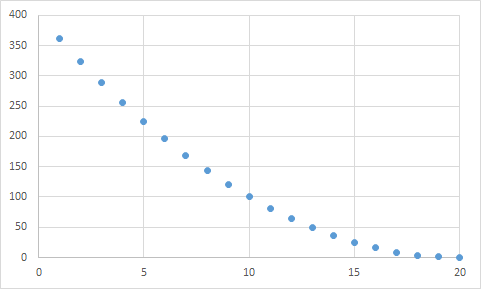
\includegraphics[scale=0.75]{satfun1}
\end{center}

\noindent
\textbf{Best-and-Worst function} \hspace{.1in} This function assumes that for the voter the difference between two candidates from the top is the same as the difference between two candidates from the bottom, while differences between candidates from the middle of the preference order are much less significant. The function is given as follows, where $m$ is the number of alternatives and $i$ is position of the alternative in the agent's preference order:

\begin{gather}
	f(x) = \frac{x^{2}+x}{2} \\
	h = \frac{m}{2} \\
	d = f(h) \\
	\alpha(i) = \begin{cases} f(h-i+1)+d-1 : i<h \\ -f(i-h)+d : i \geq h \end{cases}
\end{gather}
\\

Example of the function for $m = 20$:

\begin{center}
	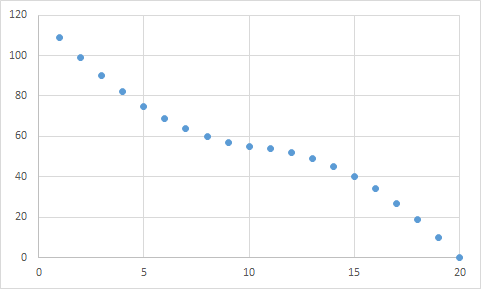
\includegraphics[scale=0.75]{satfun2}
\end{center}

\subsection{Summary of Generated Election}

Table below presents all generated test cases.

\begin{tabular}{r | c | c | c | c | c |}
	\# & alternatives count & agents count & winners count & generation model & satisfaction function \\
	\hline
	1 & \multirow{8}{*}{10} & \multirow{8}{*}{30} & \multirow{4}{*}{2} & \multirow{2}{*}{MPolya} & Square \\
	2 & & & & & Best-and-Worst \\
	\cline{5-6}
	3 & & & & \multirow{2}{*}{IC} & Square \\
	4 & & & & & Best-and-Worst \\
	\cline{4-6}
	5 & & & \multirow{4}{*}{5} & \multirow{2}{*}{MPolya} & Square \\
	6 & & & & & Best-and-Worst \\
	\cline{5-6}
	7 & & & & \multirow{2}{*}{IC} & Square \\
	8 & & & & & Best-and-Worst \\
	\hline
	9 & \multirow{8}{*}{50} & \multirow{8}{*}{400} & \multirow{4}{*}{10} & \multirow{2}{*}{MPolya} & Square \\
	10 & & & & & Best-and-Worst \\
	\cline{5-6}
	11 & & & & \multirow{2}{*}{IC} & Square \\
	12 & & & & & Best-and-Worst \\
	\cline{4-6}
	13 & & & \multirow{4}{*}{25} & \multirow{2}{*}{MPolya} & Square \\
	14 & & & & & Best-and-Worst \\
	\cline{5-6}
	15 & & & & \multirow{2}{*}{IC} & Square \\
	16 & & & & & Best-and-Worst \\
	\hline
	17 & \multirow{8}{*}{300} & \multirow{8}{*}{400} & \multirow{4}{*}{50} & \multirow{2}{*}{MPolya} & Square \\
	18 & & & & & Best-and-Worst \\
	\cline{5-6}
	19 & & & & \multirow{2}{*}{IC} & Square \\
	20 & & & & & Best-and-Worst \\
	\cline{4-6}
	21 & & & \multirow{4}{*}{200} & \multirow{2}{*}{MPolya} & Square \\
	22 & & & & & Best-and-Worst \\
	\cline{5-6}
	23 & & & & \multirow{2}{*}{IC} & Square \\
	24 & & & & & Best-and-Worst \\
	\hline
\end{tabular}
\\

\section{Test Methodology}

For each combination of problem size and generation model 100 elections were generated independently. Algorithms were evaluated against all the test files for each test case. We measured execution time and solution quality (total satisfaction) which was compared with brute-force (optimal) result for small instances and the upper bound (total satisfaction if every agent has his top alternative assigned) for medium and large instances. Execution time and solution quality are presented as an average of 100 results (with standard deviation).
\\

All test cases were used for both Chamberlin-Courant and Monroe problems.

\section{Chamberlin-Courant Problem Evaluation}

In this section we present evaluation results for Chamberlin-Courant problem.

\subsection{Small instance}

Results for small instance ($n = 30$, $m = 10$). Results are compared to optimal results.
\\

Algorithms evaluated for small instance are Algorithm C (in two versions, with $d = 10$ and $d = 15$, where $d$ is the number of functions stored), Algorithm R (with $k = 100$ computations of a random assignment), Algorithm GM, Algorithm P, Genetic Algorithm (with $I = 15$ iterations and $c = 5$ creatures) and Simulated Annealing (with initial temperature $T_{start} = 100$ and cooling rate $c = 0.1$).
\\

Results for 2 winners:
\\

\begin{tabular}{| l | r | r | r | r |}
	\hline
	\multicolumn{5}{| c |}{$n = 30$, $m = 10$, $K = 2$, Square function} \\
	\hline
	\multirow{2}{*}{algorithm} & \multicolumn{2}{c |}{MPolya} & \multicolumn{2}{c |}{IC} \\
	\cline{2-5}
	& \multicolumn{1}{c |}{time [ms]} & \multicolumn{1}{c |}{quality} & \multicolumn{1}{c |}{time [ms]} & \multicolumn{1}{c |}{quality} \\
	\hline
	C (10) & $0.66 \pm 0.12$ & $100.000 \pm 0.000 \%$ & $0.68 \pm 0.14$ & $100.000 \pm 0.000 \%$ \\
	\hline
	C (15) & $0.74 \pm 0.16$ & $100.000 \pm 0.000 \%$ & $0.74 \pm 0.14$ & $100.000 \pm 0.000 \%$ \\
	\hline
	R (100) & $0.75 \pm 0.14$ & $99.710 \pm 1.162 \%$ & $0.58 \pm 0.05$ & $99.479 \pm 1.470 \%$ \\
	\hline
	GM & $0.14 \pm 0.03$ & $99.992 \pm 0.055 \%$ & $0.10 \pm 0.02$ & $99.690 \pm 0.856 \%$ \\
	\hline
	P & $0.06 \pm 0.01$ & $87.964 \pm 8.825 \%$ & $0.05 \pm 0.02$ & $90.096 \pm 6.482 \%$ \\
	\hline
	GA (15, 5) & $0.68 \pm 0.14$ & $99.633 \pm 1.261 \%$ & $0.53 \pm 0.06$ & $99.505 \pm 1.555 \%$ \\
	\hline
	SA (100, 0.1) & $0.37 \pm 0.07$ & $98.603 \pm 2.375 \%$ & $0.28 \pm 0.04$ & $98.693 \pm 2.549 \%$ \\
	\hline
\end{tabular}

\vspace{16pt}

\begin{tabular}{| l | r | r | r | r |}
	\hline
	\multicolumn{5}{| c |}{$n = 30$, $m = 10$, $K = 2$, Best-and-Worst function} \\
	\hline
	\multirow{2}{*}{algorithm} & \multicolumn{2}{c |}{MPolya} & \multicolumn{2}{c |}{IC} \\
	\cline{2-5}
	& \multicolumn{1}{c |}{time [ms]} & \multicolumn{1}{c |}{quality} & \multicolumn{1}{c |}{time [ms]} & \multicolumn{1}{c |}{quality} \\
	\hline
	C (10) & $0.54 \pm 0.07$ & $100.000 \pm 0.000 \%$ & $0.56 \pm 0.15$ & $100.000 \pm 0.000 \%$ \\
	\hline
	C (15) & $0.56 \pm 0.06$ & $100.000 \pm 0.000 \%$ & $0.55 \pm 0.06$ & $100.000 \pm 0.000 \%$ \\
	\hline
	R (100) & $0.72 \pm 0.15$ & $99.718 \pm 1.021 \%$ & $0.59 \pm 0.07$ & $99.947 \pm 0.240 \%$ \\
	\hline
	GM & $0.16 \pm 0.03$ & $99.994 \pm 0.044 \%$ & $0.11 \pm 0.03$ & $99.414 \pm 1.375 \%$ \\
	\hline
	P & $0.06 \pm 0.01$ & $91.785 \pm 6.058 \%$ & $0.05 \pm 0.01$ & $93.725 \pm 4.245 \%$ \\
	\hline
	GA (15, 5) & $0.68 \pm 0.15$ & $99.910 \pm 0.383 \%$ & $0.52 \pm 0.05$ & $99.670 \pm 0.780 \%$ \\
	\hline
	SA (100, 0.1) & $0.32 \pm 0.05$ & $98.820 \pm 2.256 \%$ & $0.27 \pm 0.04$ & $99.144 \pm 1.778 \%$ \\
	\hline
\end{tabular}

\vspace{16pt}

Results for 5 winners:
\\

\begin{tabular}{| l | r | r | r | r |}
	\hline
	\multicolumn{5}{| c |}{$n = 30$, $m = 10$, $K = 5$, Square function} \\
	\hline
	\multirow{2}{*}{algorithm} & \multicolumn{2}{c |}{MPolya} & \multicolumn{2}{c |}{IC} \\
	\cline{2-5}
	& \multicolumn{1}{c |}{time [ms]} & \multicolumn{1}{c |}{quality} & \multicolumn{1}{c |}{time [ms]} & \multicolumn{1}{c |}{quality} \\
	\hline
	C (10) & $1.67 \pm 0.30$ & $100.000 \pm 0.000 \%$ & $1.59 \pm 0.13$ & $99.993 \pm 0.073 \%$ \\
	\hline
	C (15) & $2.29 \pm 0.52$ & $100.000 \pm 0.000 \%$ & $2.41 \pm 0.48$ & $100.000 \pm 0.000 \%$ \\
	\hline
	R (100) & $0.95 \pm 0.09$ & $99.389 \pm 0.741 \%$ & $0.94 \pm 0.07$ & $99.218 \pm 0.842 \%$ \\
	\hline
	GM & $0.16 \pm 0.02$ & $99.980 \pm 0.108 \%$ & $0.16 \pm 0.01$ & $99.534 \pm 0.738 \%$ \\
	\hline
	P & $0.06 \pm 0.01$ & $91.789 \pm 4.927 \%$ & $0.06 \pm 0.01$ & $92.450 \pm 3.546 \%$ \\
	\hline
	GA (15, 5) & $0.94 \pm 0.04$ & $99.728 \pm 0.686 \%$ & $0.97 \pm 0.05$ & $99.349 \pm 1.014 \%$ \\
	\hline
	SA (100, 0.1) & $0.53 \pm 0.04$ & $98.185 \pm 1.550 \%$ & $0.53 \pm 0.03$ & $98.323 \pm 1.464 \%$ \\
	\hline
\end{tabular}

\vspace{16pt}

\begin{tabular}{| l | r | r | r | r |}
	\hline
	\multicolumn{5}{| c |}{$n = 30$, $m = 10$, $K = 5$, Best-and-Worst function} \\
	\hline
	\multirow{2}{*}{algorithm} & \multicolumn{2}{c |}{MPolya} & \multicolumn{2}{c |}{IC} \\
	\cline{2-5}
	& \multicolumn{1}{c |}{time [ms]} & \multicolumn{1}{c |}{quality} & \multicolumn{1}{c |}{time [ms]} & \multicolumn{1}{c |}{quality} \\
	\hline
	C (10) & $1.54 \pm 0.13$ & $100.000 \pm 0.000 \%$ & $1.68 \pm 0.45$ & $100.000 \pm 0.000 \%$ \\
	\hline
	C (15) & $2.35 \pm 0.64$ & $100.000 \pm 0.000 \%$ & $2.27 \pm 0.13$ & $100.000 \pm 0.000 \%$ \\
	\hline
	R (100) & $0.93 \pm 0.08$ & $99.331 \pm 0.768 \%$ & $0.94 \pm 0.08$ & $99.425 \pm 0.632 \%$ \\
	\hline
	GM & $0.16 \pm 0.02$ & $99.982 \pm 0.091 \%$ & $0.16 \pm 0.00$ & $99.672 \pm 0.615 \%$ \\
	\hline
	P & $0.06 \pm 0.01$ & $90.235 \pm 3.734 \%$ & $0.06 \pm 0.01$ & $94.353 \pm 2.656 \%$ \\
	\hline
	GA (15, 5) & $0.96 \pm 0.10$ & $99.710 \pm 0.607 \%$ & $0.99 \pm 0.06$ & $99.621 \pm 0.544 \%$ \\
	\hline
	SA (100, 0.1) & $0.54 \pm 0.04$ & $98.431 \pm 1.350 \%$ & $0.53 \pm 0.03$ & $98.741 \pm 0.959 \%$ \\
	\hline
\end{tabular}

\subsection{Medium instance}

Results for medium instance ($n = 400$, $m = 50$). Results are compared to the upper bound.
\\

Algorithms evaluated for medium instance are Algorithm C (in two versions, with $d = 10$ and $d = 15$), Algorithm R (with $k = 100$), Algorithm GM, Algorithm P, Genetic Algorithm (in two versions, with $I = 100, c = 20$ and $I = 200, c = 25$) and Simulated Annealing (in two versions, with $T_{start} = 100, c = 0.01$ and $T_{start} = 100, c = 0.005$).
\\

\newpage

Results for 10 winners:
\\

\begin{tabular}{| l | r | r | r | r |}
	\hline
	\multicolumn{5}{| c |}{$n = 400$, $m = 50$, $K = 10$, Square function} \\
	\hline
	\multirow{2}{*}{algorithm} & \multicolumn{2}{c |}{MPolya} & \multicolumn{2}{c |}{IC} \\
	\cline{2-5}
	& \multicolumn{1}{c |}{time [ms]} & \multicolumn{1}{c |}{quality} & \multicolumn{1}{c |}{time [ms]} & \multicolumn{1}{c |}{quality} \\
	\hline
	C (10) & $251.85 \pm 11.73$ & $96.517 \pm 0.553 \%$ & $267.20 \pm 9.65$ & $89.757 \pm 0.294 \%$ \\
	\hline
	C (15) & $379.52 \pm 9.60$ & $96.517 \pm 0.553 \%$ & $402.30 \pm 9.43$ & $89.769 \pm 0.286 \%$ \\
	\hline
	R (100) & $938.14 \pm 11.43$ & $94.589 \pm 0.727 \%$ & $941.29 \pm 12.78$ & $88.540 \pm 0.224 \%$ \\
	\hline
	GM & $25.45 \pm 0.96$ & $96.508 \pm 0.591 \%$ & $27.24 \pm 2.11$ & $89.494 \pm 0.377 \%$ \\
	\hline
	P & $2.62 \pm 0.07$ & $89.795 \pm 2.308 \%$ & $2.68 \pm 0.22$ & $86.599 \pm 0.711 \%$ \\
	\hline
	GA (100, 20) & $696.82 \pm 15.81$ & $96.256 \pm 0.563 \%$ & $761.59 \pm 11.25$ & $89.412 \pm 0.315 \%$ \\
	\hline
	GA (200, 25) & $1723.27 \pm 23.67$ & $96.404 \pm 0.553 \%$ & $1894.81 \pm 19.53$ & $89.562 \pm 0.292 \%$ \\
	\hline
	SA (100, 0.01) & $169.32 \pm 7.39$ & $93.589 \pm 0.866 \%$ & $169.55 \pm 7.59$ & $88.132 \pm 0.302 \%$ \\
	\hline
	SA (100, 0.005) & $335.91 \pm 7.52$ & $94.013 \pm 0.911 \%$ & $334.44 \pm 6.37$ & $88.207 \pm 0.234 \%$ \\
	\hline
\end{tabular}

\vspace{16pt}

\begin{tabular}{| l | r | r | r | r |}
	\hline
	\multicolumn{5}{| c |}{$n = 400$, $m = 50$, $K = 10$, Best-and-Worst function} \\
	\hline
	\multirow{2}{*}{algorithm} & \multicolumn{2}{c |}{MPolya} & \multicolumn{2}{c |}{IC} \\
	\cline{2-5}
	& \multicolumn{1}{c |}{time [ms]} & \multicolumn{1}{c |}{quality} & \multicolumn{1}{c |}{time [ms]} & \multicolumn{1}{c |}{quality} \\
	\hline
	C (10) & $251.14 \pm 9.65$ & $96.733 \pm 0.510 \%$ & $266.23 \pm 9.37$ & $90.719 \pm 0.255 \%$ \\
	\hline
	C (15) & $380.68 \pm 10.18$ & $96.733 \pm 0.510 \%$ & $404.76 \pm 11.29$ & $90.731 \pm 0.247 \%$ \\
	\hline
	R (100) & $941.99 \pm 16.86$ & $95.084 \pm 0.624 \%$ & $951.27 \pm 15.43$ & $89.698 \pm 0.188 \%$ \\
	\hline
	GM & $25.56 \pm 1.46$ & $96.725 \pm 0.516 \%$ & $27.16 \pm 1.86$ & $90.529 \pm 0.323 \%$ \\
	\hline
	P & $2.61 \pm 0.07$ & $90.769 \pm 1.985 \%$ & $2.68 \pm 0.28$ & $88.062 \pm 0.600 \%$ \\
	\hline
	GA (100, 20) & $696.42 \pm 15.04$ & $96.518 \pm 0.526 \%$ & $760.18 \pm 12.71$ & $90.423 \pm 0.247 \%$ \\
	\hline
	GA (200, 25) & $1738.66 \pm 27.14$ & $96.631 \pm 0.515 \%$ & $1922.78 \pm 24.20$ & $90.554 \pm 0.261 \%$ \\
	\hline
	SA (100, 0.01) & $167.29 \pm 5.80$ & $93.988 \pm 0.739 \%$ & $167.73 \pm 7.18$ & $89.329 \pm 0.292 \%$ \\
	\hline
	SA (100, 0.005) & $338.42 \pm 10.02$ & $94.450 \pm 0.719 \%$ & $342.32 \pm 11.21$ & $89.450 \pm 0.230 \%$ \\
	\hline
\end{tabular}

\vspace{16pt}

\newpage

Results for 25 winners:
\\

\begin{tabular}{| l | r | r | r | r |}
	\hline
	\multicolumn{5}{| c |}{$n = 400$, $m = 50$, $K = 25$, Square function} \\
	\hline
	\multirow{2}{*}{algorithm} & \multicolumn{2}{c |}{MPolya} & \multicolumn{2}{c |}{IC} \\
	\cline{2-5}
	& \multicolumn{1}{c |}{time [ms]} & \multicolumn{1}{c |}{quality} & \multicolumn{1}{c |}{time [ms]} & \multicolumn{1}{c |}{quality} \\
	\hline
	C (10) & $541.20 \pm 12.76$ & $99.374 \pm 0.015 \%$ & $569.84 \pm 12.51$ & $97.585 \pm 0.119 \%$ \\
	\hline
	C (15) & $832.17 \pm 16.83$ & $99.374 \pm 0.015 \%$ & $869.71 \pm 14.88$ & $97.597 \pm 0.118 \%$ \\
	\hline
	R (100) & $2094.20 \pm 15.70$ & $98.574 \pm 0.204 \%$ & $2142.40 \pm 22.10$ & $97.041 \pm 0.084 \%$ \\
	\hline
	GM & $51.70 \pm 3.53$ & $99.373 \pm 0.146 \%$ & $54.80 \pm 3.58$ & $97.518 \pm 0.126 \%$ \\
	\hline
	P & $4.40 \pm 0.14$ & $96.740 \pm 0.855 \%$ & $4.42 \pm 0.09$ & $96.235 \pm 0.255 \%$ \\
	\hline
	GA (100, 20) & $1652.20 \pm 28.08$ & $99.138 \pm 0.183 \%$ & $1781.69 \pm 21.33$ & $97.335 \pm 0.102 \%$ \\
	\hline
	GA (200, 25) & $4096.02 \pm 60.15$ & $99.188 \pm 0.179 \%$ & $4483.16 \pm 43.37$ & $97.383 \pm 0.100 \%$ \\
	\hline
	SA (100, 0.01) & $399.24 \pm 8.47$ & $98.170 \pm 0.302 \%$ & $399.77 \pm 8.48$ & $96.859 \pm 0.113 \%$ \\
	\hline
	SA (100, 0.005) & $813.16 \pm 15.30$ & $98.326 \pm 0.252 \%$ & $813.26 \pm 14.00$ & $96.898 \pm 0.098 \%$ \\
	\hline
\end{tabular}

\vspace{16pt}

\begin{tabular}{| l | r | r | r | r |}
	\hline
	\multicolumn{5}{| c |}{$n = 400$, $m = 50$, $K = 25$, Best-and-Worst function} \\
	\hline
	\multirow{2}{*}{algorithm} & \multicolumn{2}{c |}{MPolya} & \multicolumn{2}{c |}{IC} \\
	\cline{2-5}
	& \multicolumn{1}{c |}{time [ms]} & \multicolumn{1}{c |}{quality} & \multicolumn{1}{c |}{time [ms]} & \multicolumn{1}{c |}{quality} \\
	\hline
	C (10) & $540.44 \pm 12.59$ & $99.404 \pm 0.138 \%$ & $567.23 \pm 12.07$ & $97.726 \pm 0.108 \%$ \\
	\hline
	C (15) & $831.26 \pm 18.11$ & $99.404 \pm 0.138 \%$ & $863.77 \pm 16.02$ & $97.732 \pm 0.103 \%$ \\
	\hline
	R (100) & $2136.59 \pm 23.57$ & $98.667 \pm 0.186 \%$ & $2091.77 \pm 16.60$ & $97.214 \pm 0.085 \%$ \\
	\hline
	GM & $51.68 \pm 2.23$ & $99.403 \pm 0.138 \%$ & $54.74 \pm 3.07$ & $97.662 \pm 0.118 \%$ \\
	\hline
	P & $4.39 \pm 0.25$ & $96.939 \pm 0.790 \%$ & $4.45 \pm 0.54$ & $96.472 \pm 0.233 \%$ \\
	\hline
	GA (100, 20) & $1649.14 \pm 28.84$ & $99.180 \pm 0.179 \%$ & $1769.20 \pm 19.84$ & $97.491 \pm 0.096 \%$ \\
	\hline
	GA (200, 25) & $4104.78 \pm 61.44$ & $99.227 \pm 0.172 \%$ & $4422.15 \pm 27.53$ & $97.548 \pm 0.099 \%$ \\
	\hline
	SA (100, 0.01) & $397.18 \pm 8.62$ & $98.280 \pm 0.268 \%$ & $396.13 \pm 6.25$ & $97.034 \pm 0.111 \%$ \\
	\hline
	SA (100, 0.005) & $799.15 \pm 11.14$ & $98.397 \pm 0.233 \%$ & $799.15 \pm 9.75$ & $97.090 \pm 0.105 \%$ \\
	\hline
\end{tabular}

\subsection{Large instance}

Results for large instance ($n = 400$, $m = 300$). Results are compared to the upper bound.
\\

Algorithms evaluated for large instance are Algorithm C (in two versions, with $d = 10$ and $d = 15$), Algorithm R (with $k = 100$), Algorithm GM, Algorithm P, Genetic Algorithm (in two versions, with $I = 100, c = 20$ and $I = 200, c = 25$) and Simulated Annealing (in two versions, with $T_{start} = 100, c = 0.01$ and $T_{start} = 100, c = 0.005$).
\\

\newpage

Results for 50 winners:
\\

\begin{tabular}{| l | r | r | r | r |}
	\hline
	\multicolumn{5}{| c |}{$n = 400$, $m = 300$, $K = 50$, Square function} \\
	\hline
	\multirow{2}{*}{algorithm} & \multicolumn{2}{c |}{MPolya} & \multicolumn{2}{c |}{IC} \\
	\cline{2-5}
	& \multicolumn{1}{c |}{time [s]} & \multicolumn{1}{c |}{quality} & \multicolumn{1}{c |}{time [s]} & \multicolumn{1}{c |}{quality} \\
	\hline
	C (10) & $15.66 \pm 0.11$ & $99.418 \pm 0.051 \%$ & $16.33 \pm 0.10$ & $98.466 \pm 0.056 \%$ \\
	\hline
	C (15) & $24.12 \pm 0.12$ & $99.420 \pm 0.051 \%$ & $25.04 \pm 0.14$ & $98.472 \pm 0.061 \%$ \\
	\hline
	R (100) & $0.337 \pm 0.011$ & $97.787 \pm 0.140 \%$ & $0.337 \pm 0.011$ & $97.197 \pm 0.075 \%$ \\
	\hline
	GM & $1.46 \pm 0.02$ & $99.412 \pm 0.052 \%$ & $1.53 \pm 0.02$ & $98.400 \pm 0.071 \%$ \\
	\hline
	P & $0.0585 \pm 0.0045$ & $97.029 \pm 0.416 \%$ & $0.0588 \pm 0.0049$ & $96.804 \pm 0.154 \%$ \\
	\hline
	GA (100, 20) & $6.96 \pm 0.11$ & $99.039 \pm 0.084 \%$ & $8.41 \pm 0.05$ & $97.822 \pm 0.073 \%$ \\
	\hline
	GA (200, 25) & $16.81 \pm 0.29$ & $99.125 \pm 0.069 \%$ & $20,88 \pm 0.14$ & $97.927 \pm 0.062 \%$ \\
	\hline
	SA (100, 0.01) & $1.91 \pm 0.03$ & $97.662 \pm 0.213 \%$ & $1.92 \pm 0.02$ & $97.197 \pm 0.087 \%$ \\
	\hline
	SA (100, 0.005) & $3.81 \pm 0.05$ & $97.794 \pm 0.172 \%$ & $3.85 \pm 0.03$ & $97.221 \pm 0.082 \%$ \\
	\hline
\end{tabular}

\vspace{16pt}

\begin{tabular}{| l | r | r | r | r |}
	\hline
	\multicolumn{5}{| c |}{$n = 400$, $m = 300$, $K = 50$, Best-and-Worst function} \\
	\hline
	\multirow{2}{*}{algorithm} & \multicolumn{2}{c |}{MPolya} & \multicolumn{2}{c |}{IC} \\
	\cline{2-5}
	& \multicolumn{1}{c |}{time [s]} & \multicolumn{1}{c |}{quality} & \multicolumn{1}{c |}{time [s]} & \multicolumn{1}{c |}{quality} \\
	\hline
	C (10) & $15.68 \pm 0.16$ & $99.425 \pm 0.050 \%$ & $16.32 \pm 0.10$ & $98.495 \pm 0.059 \%$ \\
	\hline
	C (15) & $24.07 \pm 0.14$ & $99.426 \pm 0.050 \%$ & $25.05 \pm 0.13$ & $98.502 \pm 0.060 \%$ \\
	\hline
	R (100) & $0.329 \pm 0.002$ & $97.838 \pm 0.129 \%$ & $0.329 \pm 0.002$ & $97.264 \pm 0.073 \%$ \\
	\hline
	GM & $1.42 \pm 0.01$ & $99.419 \pm 0.052 \%$ & $1.49 \pm 0.01$ & $98.438 \pm 0.075 \%$ \\
	\hline
	P & $0.0575 \pm 0.0006$ & $97.098 \pm 0.400 \%$ & $0.0583 \pm 0.005$ & $96.881 \pm 0.148 \%$ \\
	\hline
	GA (100, 20) & $6.79 \pm 0.10$ & $99.054 \pm 0.081 \%$ & $8.25 \pm 0.03$ & $97.872 \pm 0.069 \%$ \\
	\hline
	GA (200, 25) & $16.61 \pm 0.23$ & $99.131 \pm 0.073 \%$ & $20.50 \pm 0.42$ & $97.952 \pm 0.059 \%$ \\
	\hline
	SA (100, 0.01) & $1.89 \pm 0.03$ & $97.741 \pm 0.197 \%$ & $1.89 \pm 0.01$ & $97.239 \pm 0.092 \%$ \\
	\hline
	SA (100, 0.005) & $3.77 \pm 0.04$ & $97.840 \pm 0.175 \%$ & $3.78 \pm 0.01$ & $97.286 \pm 0.072 \%$ \\
	\hline
\end{tabular}

\vspace{16pt}

\newpage

Results for 200 winners:
\\

\begin{tabular}{| l | r | r | r | r |}
	\hline
	\multicolumn{5}{| c |}{$n = 400$, $m = 300$, $K = 200$, Square function} \\
	\hline
	\multirow{2}{*}{algorithm} & \multicolumn{2}{c |}{MPolya} & \multicolumn{2}{c |}{IC} \\
	\cline{2-5}
	& \multicolumn{1}{c |}{time [s]} & \multicolumn{1}{c |}{quality} & \multicolumn{1}{c |}{time [s]} & \multicolumn{1}{c |}{quality} \\
	\hline
	C (10) & $50.19 \pm 0.38$ & $100.000 \pm 0.000 \%$ & $50.54 \pm 0.27$ & $99.9536 \pm 0.0099 \%$ \\
	\hline
	C (15) & $79.44 \pm 0.60$ & $100.000 \pm 0.000 \%$ & $81.67 \pm 0.62$ & $99.9537 \pm 0.0097 \%$ \\
	\hline
	R (100) & $1.29 \pm 0.01$ & $99.776 \pm 0.016 \%$ & $1.29 \pm 0.00$ & $99.737 \pm 0.011 \%$ \\
	\hline
	GM & $4.04 \pm 0.02$ & $100.000 \pm 0.000 \%$ & $4.00 \pm 0.01$ & $99.952 \pm 0.010 \%$ \\
	\hline
	P & $0.134 \pm 0.002$ & $99.669 \pm 0.044 \%$ & $0.134 \pm 0.002$ & $99.672 \pm 0.031 \%$ \\
	\hline
	GA (100, 20) & $27.20 \pm 0.97$ & $100.000 \pm 0.000 \%$ & $30.67 \pm 0.08$ & $99.950 \pm 0.015 \%$ \\
	\hline
	GA (200, 25) & $67.72 \pm 2.41$ & $100.000 \pm 0.000 \%$ & $76.45 \pm 0.21$ & $99.953 \pm 0.014 \%$ \\
	\hline
	SA (100, 0.01) & $7.08 \pm 0.04$ & $99.757 \pm 0.021 \%$ & $7.05 \pm 0.02$ & $99.724 \pm 0.017 \%$ \\
	\hline
	SA (100, 0.005) & $14.16 \pm 0.06$ & $99.773 \pm 0.024 \%$ & $14.10 \pm 0.03$ & $99.736 \pm 0.014 \%$ \\
	\hline
\end{tabular}

\vspace{16pt}

\begin{tabular}{| l | r | r | r | r |}
	\hline
	\multicolumn{5}{| c |}{$n = 400$, $m = 300$, $K = 200$, Best-and-Worst function} \\
	\hline
	\multirow{2}{*}{algorithm} & \multicolumn{2}{c |}{MPolya} & \multicolumn{2}{c |}{IC} \\
	\cline{2-5}
	& \multicolumn{1}{c |}{time [s]} & \multicolumn{1}{c |}{quality} & \multicolumn{1}{c |}{time [s]} & \multicolumn{1}{c |}{quality} \\
	\hline
	C (10) & $49.33 \pm 0.35$ & $100.000 \pm 0.000 \%$ & $50.04 \pm 0.20$ & $99.9538 \pm 0.0091 \%$ \\
	\hline
	C (15) & $78.57 \pm 0.50$ & $100.000 \pm 0.000 \%$ & $80.79 \pm 0.33$ & $99.9542 \pm 0.0097 \%$ \\
	\hline
	R (100) & $1.30 \pm 0.00$ & $99.776 \pm 0.014 \%$ & $1.30 \pm 0.00$ & $99.741 \pm 0.011 \%$ \\
	\hline
	GM & $4.05 \pm 0.01$ & $100.000 \pm 0.000 \%$ & $4.00 \pm 0.01$ & $99.953 \pm 0.010 \%$ \\
	\hline
	P & $0.134 \pm 0.001$ & $99.672 \pm 0.043 \%$ & $0.134 \pm 0.001$ & $99.676 \pm 0.031 \%$ \\
	\hline
	GA (100, 20) & $27.29 \pm 0.97$ & $100.000 \pm 0.000 \%$ & $30.77 \pm 0.05$ & $99.950 \pm 0.015 \%$ \\
	\hline
	GA (200, 25) & $67.79 \pm 2.41$ & $100.000 \pm 0.000 \%$ & $77.74 \pm 0.41$ & $99.954 \pm 0.014 \%$ \\
	\hline
	SA (100, 0.01) & $7.11 \pm 0.04$ & $99.755 \pm 0.026 \%$ & $7.24 \pm 0.05$ & $99.727 \pm 0.017 \%$ \\
	\hline
	SA (100, 0.005) & $14.22 \pm 0.07$ & $99.773 \pm 0.022 \%$ & $14.32 \pm 0.11$ & $99.736 \pm 0.016 \%$ \\
	\hline
\end{tabular}

\subsection{Conclusions}

These are final conclusions regarding evaluation of algorithms for Chamberlin-Courant Problem based on all executed test cases.

\begin{enumerate}
	\item Solution quality compared to the upper bound is generally a bit better for Best-and-Worst satisfaction function. This is because for top alternatives Square function decreases faster compared to the first alternative (see chart below), so algorithms score is relatively worse when selecting second or third alternative in the preference order.
	\begin{center}
		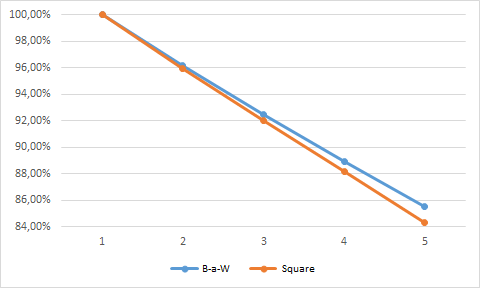
\includegraphics[scale=0.75]{satfuncomp1}
	\end{center}
	However, this is valid for all the algorithms, so differences between them are similar for both functions. It seems that the most important part of the satisfaction function is near the top of the preference order, because middle and bottom alternatives are rarely selected and differences between them are not very important, and both Square and Best-and-Worst functions are similar for the top alternatives. Results could be much different for some kind of exponential function.
	\item The difference between MPolya and IC is clearly visible for larger instances (MPolya could still be too random for smaller instances to see the difference). It is much easier to find a solution close to the upper bound for an MPolya generation model, as there is a group of alternatives that are ranked high by most agents, while IC is totally random.
	\item Algorithm C and Algorithm GM are viable for every tested case. One should use Algorithm C to get solution with the best quality possible. For many cases, increasing the number of stored functions ($d$) improves the solution quality (e.g., quality changes from 89.757\% to 89.769\% when increasing $d$ from 10 to 15 for medium instance, $K = 10$, Square function, IC), so if we seek the best solution possible, setting higher $d$ is reasonable. Algorithm GM always returns slightly weaker result than Algorithm C (or the same in case of large instance, 200 winners and MPolya, where both algorithms achieve 100\% solution quality), but it runs much faster (e.g., 4.04 seconds vs 50.19 seconds for large instance, $K = 200$, Square function, MPolya), so it may be used as a compromise between execution time and solution quality.
	\item Algorithm P returns substantially weaker solutions than Algorithm GM (e.g., 96.939\% vs 99.403\% for medium instance, $K = 25$, MPolya, Best-and-Worst function) but it runs extremely fast (4.39 ms vs 51.68 ms for the same example). It may be used if solution does not have to be very close to optimal (e.g., in recommendation systems), but there is a need to obtain it as fast as possible. This algorithm should not be used for small data sets, because the solution may be of very low quality (it has very large standard deviation for the smallest data set, which means that for some instances it returns much better result than average, but for some much worse), but this should not be a problem, because for small instances Algorithms GM runs very fast too. For larger problem, standard deviation becomes much lower and there should be no instances for which the solution quality is much worse than average.
	\item For large cases, Algorithm R can provide good results with moderate execution time (e.g., for large instance, $K = 50$, Best-and-Worst function, IC: Algorithm GM returns 98.438\% in 1.49 s, Algorithm R returns 97.264\% in 0.329 s and Algorithm P returns 96.881\% in 0.0583 s) and it is possible that this algorithm gets relatively better for even larger data sets. However, due to high level of randomization, this algorithm should only be used to supplement another one, so it can possibly find a better solution. For small and medium cases, Algorithm R does not seem to be useful. It executes longer than Algorithm C and returns worse results (e.g., for medium instance, $K = 25$, Square function, IC: Algorithm C returns 97.585\% in 569.8 ms while Algorithm R returns 97.041\% in 2142.40 ms).
    \item Genetic Algorithm and Simulated Annealing execute much too long to be useful for small and medium instances (Algorithm GM is faster and returns better results). However, Genetic Algorithm becomes much better for large data sets where there is a lot of winners. For large instance and $K = 200$, it becomes similar to Algorithm GM in means of both execution time and solution quality (e.g., for Square function, IC: Algorithm GM returns 99.952\% in 4.00 s, while Algorithm R returns 99.737\% in 1.29 s). It is possible that this algorithm may be better for even larger data sets, but it requires further research.
	\item Test cases from large instance turned out to be very easy for tested algorithms - all solutions are of very high quality compared to the upper bound. The reason of this is very high number of winners, which allows many agents to have their favourite alternative assigned, even for data generated with IC model. For MPolya and 200 winners, many algorithms always return an optimal solution which has the same total satisfaction as the upper bound - allowing 200 out of 300 candidates to win and using MPolya model allows for every agent to be maximally satisfied in virtually every case.
\end{enumerate}

\section{Monroe Problem Evaluation}

In this section we present evaluation results for Monroe problem.

\subsection{Small instance}

Results for small instance ($n = 30$, $m = 10$). Results are compared to optimal results.
\\

Algorithms evaluated for small instance are Algorithm A, Algorithm B, Algorithm C (in two versions, with $d = 10$ and $d = 15$), Algorithm R (with $k = 100$), Algorithm AR (in two versions, with $e = 0.215$, $\lambda = 0.75$ and $e = 0.015$, $\lambda = 0.9$), Algorithm GM, Genetic Algorithm (with $I = 15, c = 5$) and Simulated Annealing (with $T_{start} = 100, c = 0.1$).
\\

\newpage

Results for 2 winners:
\\

\begin{tabular}{| l | r | r | r | r |}
	\hline
	\multicolumn{5}{| c |}{$n = 30$, $m = 10$, $K = 2$, Square function} \\
	\hline
	\multirow{2}{*}{algorithm} & \multicolumn{2}{c |}{MPolya} & \multicolumn{2}{c |}{IC} \\
	\cline{2-5}
	& \multicolumn{1}{c |}{time [ms]} & \multicolumn{1}{c |}{quality} & \multicolumn{1}{c |}{time [ms]} & \multicolumn{1}{c |}{quality} \\
	\hline
	A & $0.18 \pm 0.03$ & $95.320 \pm 2.247 \%$ & $0.18 \pm 0.02$ & $94.738 \pm 2.321 \%$ \\
	\hline
	B & $0.61 \pm 0.08$ & $99.457 \pm 1.296 \%$ & $0.77 \pm 0.75$ & $99.046 \pm 1.710 \%$ \\
	\hline
	C (10) & $5.26 \pm 0.57$ & $100.000 \pm 0.000 \%$ & $5.36 \pm 0.88$ & $99.9967 \pm 0.0271 \%$ \\
	\hline
	C (15) & $7.39 \pm 0.57$ & $100.000 \pm 0.000 \%$ & $7.56 \pm 0.83$ & $99.9994 \pm 0.0063 \%$ \\
	\hline
	R (100) & $44.60 \pm 6.59$ & $99.376 \pm 2.374 \%$ & $43.26 \pm 4.16$ & $99.522 \pm 1.428 \%$ \\
	\hline
	AR (0.215, 0.75) & $20.75 \pm 2.29$ & $100.000 \pm 0.000 \%$ & $18.90 \pm 0.23$ & $100.000 \pm 0.000 \%$ \\
	\hline
	AR (0.015, 0.9) & $24.18 \pm 4.62$ & $100.000 \pm 0.000 \%$ & $21.90 \pm 5.97$ & $100.000 \pm 0.000 \%$ \\
	\hline
	GM & $6.46 \pm 1.22$ & $100.000 \pm 0.000 \%$ & $6.13 \pm 0.91$ & $99.833 \pm 0.640 \%$ \\
	\hline
	GA (15, 5) & $34.84 \pm 3.87$ & $99.352 \pm 2.259 \%$ & $34.97 \pm 4.21$ & $99.153 \pm 2.040 \%$ \\
	\hline
	SA (100, 0.1) & $19.11 \pm 0.68$ & $98.053 \pm 3.442 \%$ & $19.07 \pm 0.71$ & $98.482 \pm 2.579 \%$ \\
	\hline
\end{tabular}

\vspace{16pt}

\begin{tabular}{| l | r | r | r | r |}
	\hline
	\multicolumn{5}{| c |}{$n = 30$, $m = 10$, $K = 2$, Best-and-Worst function} \\
	\hline
	\multirow{2}{*}{algorithm} & \multicolumn{2}{c |}{MPolya} & \multicolumn{2}{c |}{IC} \\
	\cline{2-5}
	& \multicolumn{1}{c |}{time [ms]} & \multicolumn{1}{c |}{quality} & \multicolumn{1}{c |}{time [ms]} & \multicolumn{1}{c |}{quality} \\
	\hline
	A & $0.26 \pm 0.62$ & $96.872 \pm 1.604 \%$ & $0.19 \pm 0.04$ & $95.500 \pm 1.679 \%$ \\
	\hline
	B & $0.61 \pm 0.08$ & $99.581 \pm 1.019 \%$ & $0.61 \pm 0.08$ & $99.214 \pm 1.176 \%$ \\
	\hline
	C (10) & $5.41 \pm 0.77$ & $100.000 \pm 0.000 \%$ & $5.27 \pm 0.39$ & $99.980 \pm 0.152 \%$ \\
	\hline
	C (15) & $7.50 \pm 0.97$ & $100.000 \pm 0.000 \%$ & $7.63 \pm 1.42$ & $99.994 \pm 0.0062 \%$ \\
	\hline
	R (100) & $42.71 \pm 3.24$ & $99.545 \pm 2.078 \%$ & $43.32 \pm 1.69$ & $99.830 \pm 0.625 \%$ \\
	\hline
	AR (0.215, 0.75) & $22.14 \pm 5.08$ & $100.000 \pm 0.000 \%$ & $22.55 \pm 5.37$ & $100.000 \pm 0.000 \%$ \\
	\hline
	AR (0.015, 0.9) & $21.90 \pm 4.91$ & $100.000 \pm 0.000 \%$ & $22.62 \pm 5.53$ & $100.000 \pm 0.000 \%$ \\
	\hline
	GM & $5.94 \pm 0.62$ & $100.000 \pm 0.000 \%$ & $5.96 \pm 0.39$ & $99.847 \pm 0.524 \%$ \\
	\hline
	GA (15, 5) & $34.90 \pm 2.59$ & $99.662 \pm 1.274 \%$ & $35.40 \pm 4.34$ & $99.546 \pm 1.256 \%$ \\
	\hline
	SA (100, 0.1) & $19.97 \pm 2.94$ & $98.416 \pm 2.649 \%$ & $19.57 \pm 1.23$ & $99.161 \pm 1.692 \%$ \\
	\hline
\end{tabular}

\vspace{16pt}

\newpage

Results for 5 winners:
\\

\begin{tabular}{| l | r | r | r | r |}
	\hline
	\multicolumn{5}{| c |}{$n = 30$, $m = 10$, $K = 5$, Square function} \\
	\hline
	\multirow{2}{*}{algorithm} & \multicolumn{2}{c |}{MPolya} & \multicolumn{2}{c |}{IC} \\
	\cline{2-5}
	& \multicolumn{1}{c |}{time [ms]} & \multicolumn{1}{c |}{quality} & \multicolumn{1}{c |}{time [ms]} & \multicolumn{1}{c |}{quality} \\
	\hline
	A & $0.25 \pm 0.02$ & $94.065 \pm 2.307 \%$ & $0.28 \pm 0.09$ & $95.567 \pm 2.081 \%$ \\
	\hline
	B & $0.91 \pm 0.30$ & $99.296 \pm 1.231 \%$ & $0.81 \pm 0.06$ & $99.017 \pm 1.443 \%$ \\
	\hline
	C (10) & $7.78 \pm 1.64$ & $99.991 \pm 0.070 \%$ & $7.77 \pm 1.01$ & $99.918 \pm 0.366 \%$ \\
	\hline
	C (15) & $11.43 \pm 1.97$ & $100.000 \pm 0.000 \%$ & $11.56 \pm 1.56$ & $99.974 \pm 0.112 \%$ \\
	\hline
	R (100) & $55.91 \pm 5.30$ & $97.678 \pm 2.753 \%$ & $55.28 \pm 4.34$ & $99.014 \pm 1.201 \%$ \\
	\hline
	AR (0.215, 0.75) & $137.13 \pm 5.69$ & $100.000 \pm 0.000 \%$ & $136.24 \pm 6.32$ & $100.000 \pm 0.000 \%$ \\
	\hline
	AR (0.015, 0.9) & $154.83 \pm 25.07$ & $100.000 \pm 0.000 \%$ & $153.26 \pm 23.78$ & $100.000 \pm 0.000 \%$ \\
	\hline
	GM & $11.20 \pm 1.23$ & $99.946 \pm 0.240 \%$ & $11.41 \pm 1.94$ & $99.841 \pm 0.392 \%$ \\
	\hline
	GA (15, 5) & $44.28 \pm 4.15$ & $99.110 \pm 1.819 \%$ & $45.07 \pm 6.11$ & $99.276 \pm 1.158 \%$ \\
	\hline
	SA (100, 0.1) & $24.49 \pm 1.76$ & $95.158 \pm 3.961 \%$ & $24.62 \pm 2.86$ & $98.022 \pm 1.707 \%$ \\
	\hline
\end{tabular}

\vspace{16pt}

\begin{tabular}{| l | r | r | r | r |}
	\hline
	\multicolumn{5}{| c |}{$n = 30$, $m = 10$, $K = 5$, Best-and-Worst function} \\
	\hline
	\multirow{2}{*}{algorithm} & \multicolumn{2}{c |}{MPolya} & \multicolumn{2}{c |}{IC} \\
	\cline{2-5}
	& \multicolumn{1}{c |}{time [ms]} & \multicolumn{1}{c |}{quality} & \multicolumn{1}{c |}{time [ms]} & \multicolumn{1}{c |}{quality} \\
	\hline
	A & $0.26 \pm 0.01$ & $96.012 \pm 0.163 \%$ & $0.27 \pm 0.03$ & $96.864 \pm 1.589 \%$ \\
	\hline
	B & $0.79 \pm 0.07$ & $99.390 \pm 1.017 \%$ & $0.80 \pm 0.09$ & $99.251 \pm 0.997 \%$ \\
	\hline
	C (10) & $8.18 \pm 1.87$ & $99.994 \pm 0.063 \%$ & $7.83 \pm 1.06$ & $99.939 \pm 0.237 \%$ \\
	\hline
	C (15) & $11.37 \pm 2.00$ & $99.989 \pm 0.080 \%$ & $11.04 \pm 0.48$ & $99.955 \pm 0.209 \%$ \\
	\hline
	R (100) & $55.31 \pm 4.24$ & $98.508 \pm 1.602 \%$ & $54.57 \pm 4.17$ & $99.217 \pm 0.849 \%$ \\
	\hline
	AR (0.215, 0.75) & $160.17 \pm 28.16$ & $100.000 \pm 0.000 \%$ & $156.45 \pm 26.68$ & $100.000 \pm 0.000 \%$ \\
	\hline
	AR (0.015, 0.9) & $157.34 \pm 26.41$ & $100.000 \pm 0.000 \%$ & $159.08 \pm 29.08$ & $100.000 \pm 0.000 \%$ \\
	\hline
	GM & $10.96 \pm 1.07$ & $99.971 \pm 0.158 \%$ & $11.15 \pm 1.74$ & $99.921 \pm 0.200 \%$ \\
	\hline
	GA (15, 5) & $44.08 \pm 4.53$ & $99.458 \pm 1.048 \%$ & $44.45 \pm 4.90$ & $99.601 \pm 0.715 \%$ \\
	\hline
	SA (100, 0.1) & $24.84 \pm 3.14$ & $96.261 \pm 2.710 \%$ & $24.70 \pm 2.93$ & $98.591 \pm 1.111 \%$ \\
	\hline
\end{tabular}

\subsection{Medium instance}

Results for medium instance ($n = 400$, $m = 50$). Results are compared to the upper bound.
\\

Algorithms evaluated for medium instance are Algorithm A, Algorithm B, Algorithm C (in two versions, with $d = 10$ and $d = 15$), Algorithm R (with $k = 100$) and Algorithm AR (with $e = 0.215$, $\lambda = 0.75$).
\\

\newpage

Algorithm GM, Genetic Algorithm and Simulated Annealing have been omitted from results for this case, as their execution time is too long. These are example results for one execution of each algorithm (10 winners, MPolya, Square function):
\\

\begin{tabular}{| l | c | c |}
	\hline
	algorithm & time [s] & quality \\
	\hline
	GM & $207.70$ & $95.467 \%$ \\
	\hline
	GA (100, 20) & $>300$ (timeout) & - \\
	\hline
	SA (100, 0.01) & $>300$ (timeout) & - \\
	\hline
\end{tabular}

\vspace{16pt}

Results for 10 winners:
\\

\begin{tabular}{| l | r | r | r | r |}
	\hline
	\multicolumn{5}{| c |}{$n = 400$, $m = 50$, $K = 10$, Square function} \\
	\hline
	\multirow{2}{*}{algorithm} & \multicolumn{2}{c |}{MPolya} & \multicolumn{2}{c |}{IC} \\
	\cline{2-5}
	& \multicolumn{1}{c |}{time [s]} & \multicolumn{1}{c |}{quality} & \multicolumn{1}{c |}{time [s]} & \multicolumn{1}{c |}{quality} \\
	\hline
	A & $0.0827 \pm 0.0065$ & $90.515 \pm 0.843 \%$ & $0.0814 \pm 0.0041$ & $83.825 \pm 0.417 \%$ \\
	\hline
	B & $0.860 \pm 0.023$ & $95.529 \pm 0.526 \%$ & $0.848 \pm 0.014$ & $88.975 \pm 0.400 \%$ \\
	\hline
	C (10) & $9.91 \pm 0.44$ & $95.684 \pm 0.504 \%$ & $9.76 \pm 0.42$ & $89.390 \pm 0.317 \%$ \\
	\hline
	C (15) & $14.83 \pm 0.62$ & $95.692 \pm 0.505 \%$ & $14.55 \pm 0.53$ & $89.442 \pm 0.305 \%$ \\
	\hline
	R (100) & $7.88 \pm 0.07$ & $84.923 \pm 2.476 \%$ & $7.68 \pm 0.06$ & $87.006 \pm 0.400 \%$ \\
	\hline
	AR (0.215, 0.75) & $11.87 \pm 0.07$ & $90.536 \pm 0.834 \%$ & $11.52 \pm 0.07$ & $87.011 \pm 0.406 \%$ \\
	\hline
\end{tabular}

\vspace{16pt}

\begin{tabular}{| l | r | r | r | r |}
	\hline
	\multicolumn{5}{| c |}{$n = 400$, $m = 50$, $K = 10$, Best-and-Worst function} \\
	\hline
	\multirow{2}{*}{algorithm} & \multicolumn{2}{c |}{MPolya} & \multicolumn{2}{c |}{IC} \\
	\cline{2-5}
	& \multicolumn{1}{c |}{time [s]} & \multicolumn{1}{c |}{quality} & \multicolumn{1}{c |}{time [s]} & \multicolumn{1}{c |}{quality} \\
	\hline
	A & $0.0796 \pm 0.0035$ & $92.016 \pm 0.696 \%$ & $0.0840 \pm 0.0077$ & $86.296 \pm 0.324 \%$ \\
	\hline
	B & $0.849 \pm 0.016$ & $95.823 \pm 0.498 \%$ & $0.854 \pm 0.017$ & $90.070 \pm 0.343 \%$ \\
	\hline
	C (10) & $9.86 \pm 0.42$ & $95.966 \pm 0.457 \%$ & $9.70 \pm 0.43$ & $90.402 \pm 0.271 \%$ \\
	\hline
	C (15) & $14.75 \pm 0.51$ & $95.975 \pm 0.466 \%$ & $14.57 \pm 0.55$ & $90.449 \pm 0.271 \%$ \\
	\hline
	R (100) & $7.86 \pm 0.06$ & $87.006 \pm 2.160 \%$ & $7.71 \pm 0.07$ & $88.384 \pm 0.325 \%$ \\
	\hline
	AR (0.215, 0.75) & $11.85 \pm 0.07$ & $92.023 \pm 0.694 \%$ & $11.66 \pm 0.09$ & $88.483 \pm 0.316 \%$ \\
	\hline
\end{tabular}

\vspace{16pt}

\newpage

Results for 25 winners:
\\

\begin{tabular}{| l | r | r | r | r |}
	\hline
	\multicolumn{5}{| c |}{$n = 400$, $m = 50$, $K = 25$, Square function} \\
	\hline
	\multirow{2}{*}{algorithm} & \multicolumn{2}{c |}{MPolya} & \multicolumn{2}{c |}{IC} \\
	\cline{2-5}
	& \multicolumn{1}{c |}{time [s]} & \multicolumn{1}{c |}{quality} & \multicolumn{1}{c |}{time [s]} & \multicolumn{1}{c |}{quality} \\
	\hline
	A & $0.171 \pm 0.005$ & $93.475 \pm 0.721 \%$ & $0.169 \pm 0.006$ & $93.920 \pm 0.296 \%$ \\
	\hline
	B & $1.03 \pm 0.02$ & $97.814 \pm 0.363 \%$ & $1.03 \pm 0.02$ & $97.023 \pm 0.139 \%$ \\
	\hline
	C (10) & $12.00 \pm 0.56$ & $97.957 \pm 0.325 \%$ & $12.04 \pm 0.53$ & $97.165 \pm 0.131 \%$ \\
	\hline
	C (15) & $18.04 \pm 0.72$ & $97.966 \pm 0.324 \%$ & $18.11 \pm 0.69$ & $97.181 \pm 0.127 \%$ \\
	\hline
	R (100) & $8.81 \pm 0.08$ & $91.197 \pm 1.900 \%$ & $8.56 \pm 0.05$ & $96.111 \pm 0.150 \%$ \\
	\hline
	AR (0.215, 0.75) & $13.81 \pm 0.72$ & $93.572 \pm 0.705 \%$ & $13.02 \pm 0.08$ & $96.144 \pm 0.133 \%$ \\
	\hline
\end{tabular}

\vspace{16pt}

\begin{tabular}{| l | r | r | r | r |}
	\hline
	\multicolumn{5}{| c |}{$n = 400$, $m = 50$, $K = 25$, Best-and-Worst function} \\
	\hline
	\multirow{2}{*}{algorithm} & \multicolumn{2}{c |}{MPolya} & \multicolumn{2}{c |}{IC} \\
	\cline{2-5}
	& \multicolumn{1}{c |}{time [s]} & \multicolumn{1}{c |}{quality} & \multicolumn{1}{c |}{time [s]} & \multicolumn{1}{c |}{quality} \\
	\hline
	A & $0.171 \pm 0.008$ & $94.525 \pm 0.597 \%$ & $0.169 \pm 0.006$ & $94.754 \pm 0.225 \%$ \\
	\hline
	B & $1.04 \pm 0.02$ & $97.936 \pm 0.345 \%$ & $1.04 \pm 0.02$ & $97.200 \pm 0.141 \%$ \\
	\hline
	C (10) & $12.04 \pm 0.56$ & $98.068 \pm 0.306 \%$ & $12.11 \pm 0.55$ & $97.334 \pm 0.126 \%$ \\
	\hline
	C (15) & $18.04 \pm 0.66$ & $98.080 \pm 0.306 \%$ & $18.08 \pm 0.67$ & $97.349 \pm 0.121 \%$ \\
	\hline
	R (100) & $8.82 \pm 0.07$ & $92.322 \pm 1.405 \%$ & $8.58 \pm 0.09$ & $96.345 \pm 0.144 \%$ \\
	\hline
	AR (0.215, 0.75) & $13.48 \pm 0.13$ & $94.542 \pm 0.583 \%$ & $13.06 \pm 0.09$ & $96.393 \pm 0.141 \%$ \\
	\hline
\end{tabular}

\subsection{Large instance}

Results for large instance ($n = 400$, $m = 300$). Results are compared to the upper bound.
\\

Algorithms evaluated for large instance are Algorithm A, Algorithm B, Algorithm C (with $d = 5$), Algorithm R (with $k = 10$) and Algorithm AR (with $e = 0.215$, $\lambda = 0.75$).
\\

Parameters of algorithms C and R were adjusted to maintain reasonable execution time.
\\

\newpage

Results for 50 winners:
\\

\begin{tabular}{| l | r | r | r | r |}
	\hline
	\multicolumn{5}{| c |}{$n = 400$, $m = 300$, $K = 50$, Square function} \\
	\hline
	\multirow{2}{*}{algorithm} & \multicolumn{2}{c |}{MPolya} & \multicolumn{2}{c |}{IC} \\
	\cline{2-5}
	& \multicolumn{1}{c |}{time [s]} & \multicolumn{1}{c |}{quality} & \multicolumn{1}{c |}{time [s]} & \multicolumn{1}{c |}{quality} \\
	\hline
	A & $7.77 \pm 0.04$ & $97.894 \pm 0.120 \%$ & $7.66 \pm 0.03$ & $96.944 \pm 0.127 \%$ \\
	\hline
	B & $8.81 \pm 0.06$ & $99.103 \pm 0.062 \%$ & $8.67 \pm 0.04$ & $98.170 \pm 0.077 \%$ \\
	\hline
	C (5) & $45.65 \pm 0.50$ & $99.131 \pm 0.059 \%$ & $45.17 \pm 0.40$ & $98.224 \pm 0.063 \%$ \\
	\hline
	R (10) & $10.41 \pm 0.10$ & $93.630 \pm 0.915 \%$ & $10.11 \pm 0.09$ & $96.724 \pm 0.089 \%$ \\
	\hline
	AR (0.215, 0.75) & $23.41 \pm 0.14$ & $97.894 \pm 0.120 \%$ & $22.84 \pm 0.19$ & $96.954 \pm 0.120 \%$ \\
	\hline
\end{tabular}

\vspace{16pt}

\begin{tabular}{| l | r | r | r | r |}
	\hline
	\multicolumn{5}{| c |}{$n = 400$, $m = 300$, $K = 50$, Best-and-Worst function} \\
	\hline
	\multirow{2}{*}{algorithm} & \multicolumn{2}{c |}{MPolya} & \multicolumn{2}{c |}{IC} \\
	\cline{2-5}
	& \multicolumn{1}{c |}{time [s]} & \multicolumn{1}{c |}{quality} & \multicolumn{1}{c |}{time [s]} & \multicolumn{1}{c |}{quality} \\
	\hline
	A & $7.74 \pm 0.04$ & $98.048 \pm 0.104 \%$ & $7.60 \pm 0.04$ & $97.175 \pm 0.106 \%$ \\
	\hline
	B & $8.78 \pm 0.05$ & $99.118 \pm 0.060 \%$ & $8.58 \pm 0.02$ & $98.205 \pm 0.074 \%$ \\
	\hline
	C (5) & $45.95 \pm 0.58$ & $99.141 \pm 0.058 \%$ & $45.47 \pm 0.57$ & $98.258 \pm 0.063 \%$ \\
	\hline
	R (10) & $10.58 \pm 0.09$ & $93.955 \pm 0.670 \%$ & $10.01 \pm 0.10$ & $96.806 \pm 0.087 \%$ \\
	\hline
	AR (0.215, 0.75) & $23.87 \pm 0.19$ & $98.048 \pm 0.104 \%$ & $22.56 \pm 0.13$ & $97.175 \pm 0.106 \%$ \\
	\hline
\end{tabular}

\vspace{16pt}

\newpage

Results for 200 winners:
\\

\begin{tabular}{| l | r | r | r | r |}
	\hline
	\multicolumn{5}{| c |}{$n = 400$, $m = 300$, $K = 200$, Square function} \\
	\hline
	\multirow{2}{*}{algorithm} & \multicolumn{2}{c |}{MPolya} & \multicolumn{2}{c |}{IC} \\
	\cline{2-5}
	& \multicolumn{1}{c |}{time [s]} & \multicolumn{1}{c |}{quality} & \multicolumn{1}{c |}{time [s]} & \multicolumn{1}{c |}{quality} \\
	\hline
	A & $26.23 \pm 0.11$ & $98.417 \pm 0.156 \%$ & $25.19 \pm 0.08$ & $99.423 \pm 0.053 \%$ \\
	\hline
	B & $28.71 \pm 0.15$ & $99.380 \pm 0.056 \%$ & $27.67 \pm 0.10$ & $99.683 \pm 0.019 \%$ \\
	\hline
	C (5) & $145.10 \pm 10.83$ & $99.395 \pm 0.056 \%$ & $138.29 \pm 11.62$ & $99.693 \pm 0.017 \%$ \\
	\hline
	R (10) & $26.06 \pm 0.25$ & $97.284 \pm 0.397 \%$ & $26.25 \pm 0.41$ & $99.320 \pm 0.028 \%$ \\
	\hline
	AR (0.215, 0.75) & $65.38 \pm 0.40$ & $98.417 \pm 0.155 \%$ & $65.00 \pm 0.41$ & $99.425 \pm 0.050 \%$ \\
	\hline
\end{tabular}

\vspace{16pt}

\begin{tabular}{| l | r | r | r | r |}
	\hline
	\multicolumn{5}{| c |}{$n = 400$, $m = 300$, $K = 200$, Square function} \\
	\hline
	\multirow{2}{*}{algorithm} & \multicolumn{2}{c |}{MPolya} & \multicolumn{2}{c |}{IC} \\
	\cline{2-5}
	& \multicolumn{1}{c |}{time [s]} & \multicolumn{1}{c |}{quality} & \multicolumn{1}{c |}{time [s]} & \multicolumn{1}{c |}{quality} \\
	\hline
	A & $25.86 \pm 0.11$ & $98.497 \pm 0.140 \%$ & $24.81 \pm 0.06$ & $99.438 \pm 0.049 \%$ \\
	\hline
	B & $28.30 \pm 0.12$ & $99.387 \pm 0.057 \%$ & $27.21 \pm 0.08$ & $99.686 \pm 0.019 \%$ \\
	\hline
	C (5) & $144.59 \pm 10.79$ & $99.402 \pm 0.055 \%$ & $138.02 \pm 11.48$ & $99.696 \pm 0.017 \%$ \\
	\hline
	R (10) & $25.69 \pm 0.26$ & $97.423 \pm 0.308 \%$ & $25.55 \pm 0.21$ & $99.328 \pm 0.027 \%$ \\
	\hline
	AR (0.215, 0.75) & $64.05 \pm 0.43$ & $98.497 \pm 0.140 \%$ & $63.16 \pm 0.51$ & $99.439 \pm 0.048 \%$ \\
	\hline
\end{tabular}

\subsection{Conclusions}

These are final conclusions regarding evaluation of algorithms for Monroe Problem based on all executed test cases.

\begin{enumerate}
	\item For most cases algorithms generally return a bit higher satisfaction for the Best-and-Worst function than for the Square function. It is caused by the fact that Square function is decreasing relatively faster for top alternatives (as described in section 4.4.4). However, differences between the algorithms are similar, the same as for Chamberlin-Courant problem. Using much different function, e.g. an exponential one, could potentially change the results.
	\item Generally, algorithms achieve higher solution quality for data generated with MPolya (especially with less winners). This is an expected behaviour, as with MPolya it is easier to include more candidates from the top in the solution. The only exception to this rule is Algorithm R. It may be caused by high randomization of IC data, which causes random solutions to be relatively better.
	\item Algorithm C seems to be the best and universal option to attain a very high quality solution for most cases. It is sometimes a bit worse than Algorithm AR for the small instance (e.g. 99.994\% vs 100\% for $K = 2$, Best-and-Worst function, IC), but runs much faster (7.63 ms vs 22.55 ms for the same case). It can be also adjusted to one's needs by modifying number of stored functions (parameter $d$) and in many cases it improves the solution quality (e.g. for medium instance, $K = 10$, Square function, IC, quality changes from 89.390\% to 89.442\% after increasing $d$ from 10 to 15).
	\item Quality of solution generated by Algorithm B is always significantly lower than the one generated by Algorithm C (e.g. 90.070\% vs 90.402\% for medium instance, $K = 10$, Best-and-Worst function, IC), but the algorithm itself is much faster (0.854 s vs 9.70 s for the same case). It may be seen as a trade-off between solution quality and execution time.
	\item For small and medium cases, Algorithm A may be a good option for some appliances, as it returns result very fast. Its quality is far from optimal, but there may be some systems where it is not as important as execution time. For larger instances, it is better to use Algorithm B instead, as difference in execution time becomes relatively lower when we increase problem size (e.g. 7.60 s vs 8.58 s for large instance, $K = 50$, Best-and-Worst function, IC), because for larger cases reassignment of agents, which is the only difference between the algorithms, becomes less significant.
	\item Algorithm AR gives the best quality of solution among tested algorithms for the small instance, but it is very slow. It seems to be underperforming for larger instances - other algorithms give better solutions faster. Maybe changing parameters could help, but it would further increase execution time.
    \item Algorithm R is not a good choice, because for each case there is an algorithm that returns better solution in shorter time.
	\item Quality of solution returned by algorithms for the large instance is extremely high compared to the upper bound. The reason is that number of winners is very high compared to number of agents ($50/400$, $200/400$) and to the number of alternatives ($50/300$, $200/300$). Such situation allows to assign favourite alternatives to most agents, especially with data generated by MPolya.
\end{enumerate}
\chapter{Summary}
\label{cha:testy}

We have found that for both Chamberlin-Courant and Monroe problems there are algorithms that perform very well under nonlinear satisfaction function. Algorithm C is especially interesting (for both problems), because it attains solutions of very good quality for every tested data set (very often close to optimal or upper bound) and at the same time it can be tuned (by changing its input parameter) to try to find even better solution if we can afford longer execution time.

At the same time, there are excellent algorithms that can be used if we want good but not necessarily best possible solution, but we have limited time. This may be the case for some software systems.

We have shown that heuristic algorithms (Genetic Algorithm and Simulated Annealing) do not fit CC and Monroe problems well. They can provide solutions of good quality, but execution time is too long.

\section{Further Research}

These are main areas of potential further research:
\begin{enumerate}
	\item Using different satisfaction function could change the results. We have not tested algorithms against any function where differences between top alternatives would be much greater (e.g., exponential function). It would surely make quality of solutions much lower compared to upper bound and could potentially favour different algorithms.
	\item Testing algorithms against different combinations of number of alternatives, number of agents and number of winner could also provide some interesting data. As we have seen for the largest tested instance, results vary a lot when ratio between these three parameters is adjusted.
\end{enumerate}

% itd.
% \appendix
% \include{dodatekA}
% \include{dodatekB}
% itd.



\bibliography{bibliography}
\bibliographystyle{unsrt}

\addcontentsline{toc}{chapter}{\listtablename}
\listoftables

\end{document}
